\section{Analysis Stuff}
\begin{definition*}[Derivative and integration rules]
  Linearity: \((\alpha \cdot f(x) + g(x))' = \alpha \cdot f'(x) + g'(x)\) \\
  Product rule: \((f \cdot g)'(x) = f'(x)\cdot g(x) + f(x)\cdot g'(x)\) \\
  Quotient rule: \(\left(\frac{f}{g}\right)'(x) = \frac{f'(x)\cdot g(x) - f(x)\cdot g'(x)}{g(x)^2}\) \\
  Chain rule: \((f \circ g)'(x) = f'(g(x))\cdot g'(x)\) \\
  Inverse: \((f^{-1})'(y_0) = \frac{1}{f'(x_0)} = \frac{1}{f'(f^{-1}(y_0))}, \ y_0 = f(x_0)\) \\
  Part. Int.: \(\int f(x) g'(x) \,dx = f(x)g(x) - \int f'(x) g(x) \, dx\)
\end{definition*}

\begin{itemize}
    \item Choose $g'$: exp $\rightarrow$ trig $\rightarrow$ poly $\rightarrow$ inverse trig. $\rightarrow$ logs
    \item Choose $f$: logs $\rightarrow$ inverse trig. $\rightarrow$ poly $\rightarrow$ trig $\rightarrow$ exp
    \item Sometimes it is necessary to multiply by $1$. \\ E.g.: $\int \ln x \ \,dx = \int \ln x \cdot 1 \ \,dx \Rightarrow f(x) = \ln x, \ g'(x) = 1$.
\end{itemize}

\begin{definition*}[Substitution] \vspace{-7pt}
    \[\int_{\phi(a)}^{\phi(b)} f(x) \,dx = \int_a^b f(\phi(t)) \phi'(t) dt = (F \circ \phi)(b) - (F \circ \phi)(a)\]
    since $F'=f$ then $f(\phi(t))\phi'(t) = (F \circ \phi)'(t)$.
\end{definition*}

\subsection{Series}
\begin{itemize}
  \item Geometric: $\sum_{n = 0}^\infty q^n = \frac{1}{1 - q}$ if $|q| < 1$
  \item Harmonic: $\sum_{n = 1}^\infty \frac{1}{n}$ diverges
  \item Telescope: $\sum_{n = 0}^\infty \frac{1}{n(n + 1)} = 1$
  \item $\exp(z) := \sum_{n = 0}^\infty \frac{z^n}{n!} = \lim_{n\to\infty}(1 + \frac{z}{n})^n = e^z$
  \item $\zeta(s) = \sum_{n=1}^\infty \frac{1}{n^s}$ converges $s > 1 \ (\frac{1}{1 - \frac{1}{2^{s-1}}})$
  \item $\text{p}(z) = \sum_{k = 0}^\infty c_kz^k$ conv. abs. $|z| < \rho = \frac{1}{\limsup |c_k|^{1/k}}$
\end{itemize}
\begin{tabularx}{\linewidth}{XX}
  \toprule
  $\sum\limits_{i=1}^n i = \frac{n(n+1)}{2}$ & $\sum\limits_{i=1}^n i^2 = \frac{n(n+1)(2n + 1)}{6}$ \\
  $\sum\limits_{i=1}^n i^3 = \frac{n^2(n+1)^2}{4}$ & $\sum\limits_{i=1}^\infty \frac{1}{n^2} = \frac{\pi^2}{6}$ \\
  \bottomrule
\end{tabularx}

\subsection{Logarithm Rules}
\renewcommand{\arraystretch}{1}
\begin{tabularx}{\linewidth}{XX}
  $\ln(1) = 0$ & $\ln(e) = 1$ \\
  $\ln(xy) = \ln(x) + \ln(y)$ & $\ln(x/y) = \ln(x) - \ln(y)$ \\
  $\ln(x^y) = y \cdot \ln(x)$ & $x^\alpha \cdot x^\beta = x^{\alpha + \beta}$ \\
  $(x^\alpha)^\beta = x^{\alpha \cdot \beta}$ & $\frac{x - 1}{x} \leq \ln(x) \leq x - 1$ \\
  $\ln(1 + x^\alpha) \leq \alpha x$ & $\log_\alpha(x) = \frac{\ln(x)}{\ln(\alpha)}$
\end{tabularx}

\subsection{Important Functions}
\begin{center}
  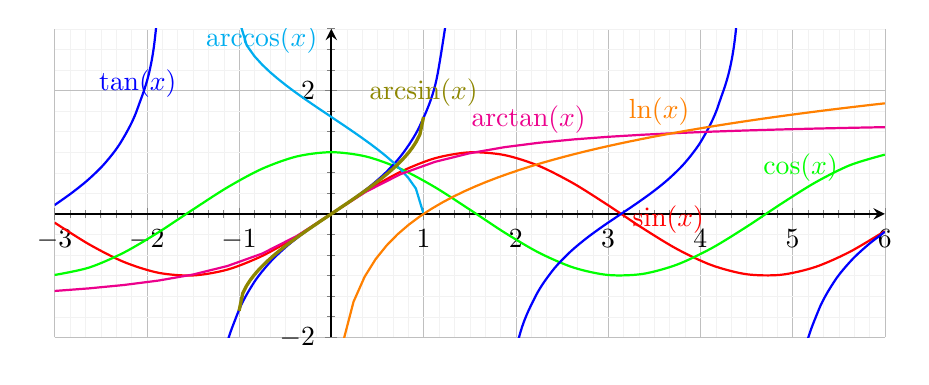
\begin{tikzpicture}
      \begin{axis}[
          axis lines = middle,
          domain = -3:6,
          ymin = -2,
          ymax = 3,
          width = \linewidth,
          height = 5.5cm,
          style = thick,
          grid = both,
          grid style = {line width=.1pt, draw=gray!10},
          major grid style = {line width=.2pt,draw=gray!50},
          minor tick num = 5,
          restrict y to domain=-10:10,
      ]
      
      \addplot[red, smooth]{sin(deg(x))} node[pos=0.75] (endofplotsquare1) {};
      \node [above,color=red] at (endofplotsquare1) {$\sin(x)$};

      \addplot[green, smooth]{cos(deg(x))} node[pos=0.9] (endofplotsquare2) {};
      \node [above,color=green] at (endofplotsquare2) {$\cos(x)$};

      \addplot[blue, smooth, samples=51]{tan(deg(x))} node[pos=0.05] (endofplotsquare3) {};
      \node [above,color=blue] at (endofplotsquare3) {$\tan(x)$};
      
      \addplot[cyan, domain=-1:1]{acos(x)/180*pi} node[pos=0.2] (endofplotsquare4) {};
      \node [above,color=cyan] at (endofplotsquare4) {$\arccos(x)$};

      \addplot[magenta] {atan(x)/180*pi} node[pos=0.6] (endofplotsquare5) {};
      \node [above,color=magenta] at (endofplotsquare5) {$\arctan(x)$};

      \addplot[olive, domain=-1:1, samples=51, style=very thick]{asin(x)/180*pi} node[pos=1] (endofplotsquare6) {};
      \node [above,color=olive] at (endofplotsquare6) {$\arcsin(x)$};

      \addplot[orange, domain=0.001:6, samples=51]{ln(x)} node[pos=0.8] (endofplotsquare7) {};
      \node [above,color=orange] at (endofplotsquare7) {$\ln(x)$};

      \end{axis}
  \end{tikzpicture}
\end{center}

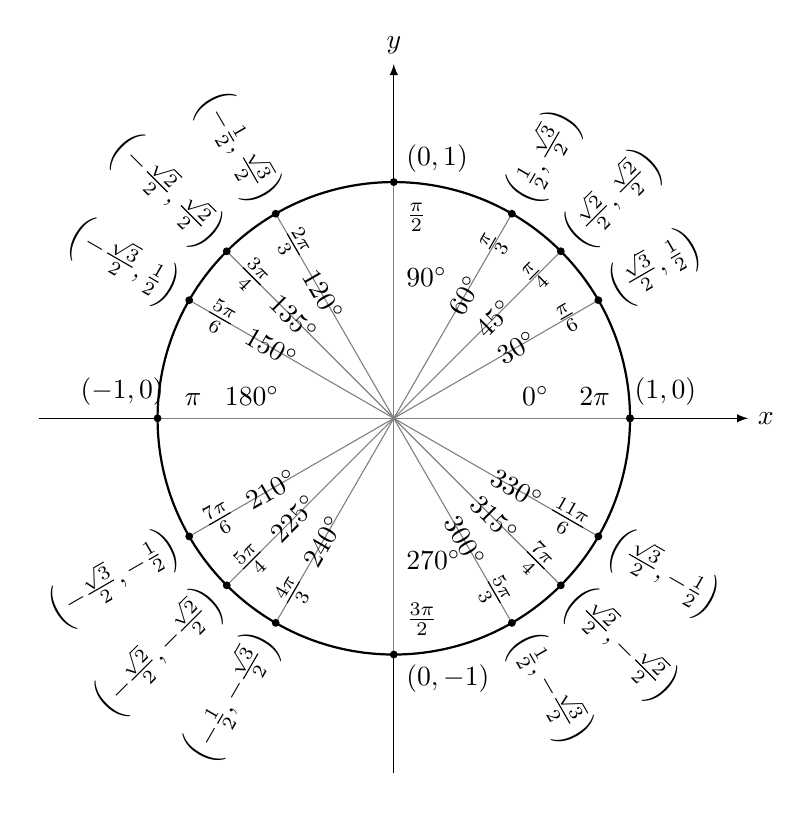
\begin{tikzpicture}[scale=3,cap=round,>=latex]
  \draw[->] (-1.5cm,0cm) -- (1.5cm,0cm) node[right,fill=white] {$x$}; % x axis
  \draw[->] (0cm,-1.5cm) -- (0cm,1.5cm) node[above,fill=white] {$y$}; % y axis
  
  % draw the unit circle
  \draw[thick] (0cm,0cm) circle(1cm);
  
  \foreach \x in {45,135, 225,315,0,30,...,360} { % <-- bissectrices added
    \draw[gray] (0cm,0cm) -- (\x:1cm); % lines from center to point
    \filldraw[black] (\x:1cm) circle(0.4pt); % dots at each point
  }
  
  % for the first and fourth quadrants
  \foreach \adeg/\radtext/\xc/\yc in {
    30/\frac{\pi}{6}/\frac{\sqrt{3}}{2}/\frac{1}{2},
    45/\frac{\pi}{4}/\frac{\sqrt{2}}{2}/\frac{\sqrt{2}}{2},
    60/\frac{\pi}{3}/\frac{1}{2}/\frac{\sqrt{3}}{2},
    300/\frac{5\pi}{3}/\frac{1}{2}/-\frac{\sqrt{3}}{2},
    315/\frac{7\pi}{4}/\frac{\sqrt{2}}{2}/-\frac{\sqrt{2}}{2},
    330/\frac{11\pi}{6}/\frac{\sqrt{3}}{2}/-\frac{1}{2}
  }
  {
    \draw (\adeg:0.6cm) node[rotate around={\adeg:(0,0)}] {$\adeg^\circ$}; % <-- rotate around key used
    \draw (\adeg:0.85cm) node[rotate around={\adeg:(0,0)}] {$\radtext$}; % <-- rotate around key used
    \draw (\adeg:1.025cm) node[rotate around={\adeg:(0,0)}, anchor=west] {$\left(\xc,\yc\right)$}; % <-- rotate around key used, radius changed, anchor key used
  }

  % for the second and third quadrants
  \foreach \adeg/\radtext/\xc/\yc in {
    120 / \frac{2\pi}{3} / -\frac{1}{2} / \frac{\sqrt{3}}{2},
    135 / \frac{3\pi}{4} / -\frac{\sqrt{2}}{2} / \frac{\sqrt{2}}{2},
    150 / \frac{5\pi}{6} / -\frac{\sqrt{3}}{2} / \frac{1}{2},
    210 / \frac{7\pi}{6} / -\frac{\sqrt{3}}{2} / -\frac{1}{2},
    225 / \frac{5\pi}{4} / -\frac{\sqrt{2}}{2} / -\frac{\sqrt{2}}{2},
    240 / \frac{4\pi}{3} / -\frac{1}{2} / -\frac{\sqrt{3}}{2}
  }
  {
    \draw (\adeg:0.6cm) node[rotate around={\adeg+180:(0,0)}] {$\adeg^\circ$}; % <-- rotate around key used
    \draw (\adeg:0.85cm) node[rotate around={\adeg+180:(0,0)}] {$\radtext$}; % <-- rotate around key used
    \draw (\adeg:1.025cm) node[rotate around={\adeg+180:(0,0)}, anchor=east] {$\left(\xc,\yc\right)$}; % <-- rotate around key used, radius changed, anchor key used
  }
  
  \foreach \adeg/\radtext/\xc/\yc in {0 / 2\pi / 1 / 0, 180 / \pi / -1 / 0}
  {
    \draw (\adeg:0.6cm) node[above=1pt] {$\adeg^\circ$};
    \draw (\adeg:0.85cm) node[above=1pt] {$\radtext$};
    \draw (\adeg:1.15cm) node[above=1pt] {$\left(\xc,\yc\right)$}; % <-- radius changed
  }
  
  \foreach \adeg/\radtext/\xc/\yc in {90 / \frac{\pi}{2} / 0 / 1, 270 / \frac{3\pi}{2} / 0 / -1}
  {
    \draw (\adeg:0.6cm) node[right=1pt] {$\adeg^\circ$};
    \draw (\adeg:0.85cm) node[right=1pt] {$\radtext$};
    \draw (\adeg:1.1cm) node[right=1pt] {$\left(\xc,\yc\right)$}; % <-- radius changed
  }
\end{tikzpicture}

\begin{center}
  \begin{tabular}{cc}
    \(\binom{n}{k} = \frac{n!}{(n-k)!k!}\) & \((x + y)^n = \sum\limits_{k=0}^n \binom{n}{k}x^{n-k}y^k\) \\
    \(x = \frac{-b \pm \sqrt{b^2 - 4ac}}{2a}\)
  \end{tabular}
\end{center}

\subsection*{Derivatives and Integrals (\href{https://n.ethz.ch/~dcamenisch/summaries/}{src: dcamenisch})}
\renewcommand{\arraystretch}{1.5}
\begin{center}
\begin{tabular}{c|c}
    $\mathbf{F(x)}$ & $\mathbf{f(x)}$ \\
    \midrule
    $c$ & $0$ \\
    $x^a$ & $a \cdot x^{a - 1}$ \\
    $\frac{1}{a+1} x^{a + 1}$ & $x^a$ \\
    $\frac{1}{a \cdot (n + 1)} (ax + b)^{n + 1}$ & $(ax + b)^n$ \\
    $\frac{x^{a + 1}}{a + 1}$ & $x^a, \ a \neq -1$ \\
    $\frac{1}{x}$ & $-\frac{1}{x^2}$ \\
    $\sqrt{x}$ & $\frac{1}{2\sqrt{x}}$ \\
    $\sqrt[n]{x}$ & $\frac{1}{n}x^{\frac{1}{n} - 1}$ \\
    $\frac{2}{3}x^{\frac{3}{2}}$ & $\sqrt{x}$ \\
    $\frac{n}{n+1} x^{\frac{1}{n} + 1}$ & $\sqrt[n]{x}$ \\
    $e^x$ & $e^x$ \\
    $\ln(|x|)$ & $\frac{1}{x}$ \\
    $\log_a(|x|)$ & $\frac{1}{x \ln(a)} = \log_a(e^\frac{1}{x})$ \\
    $\sin(x)$ & $\cos(x)$ \\
    $\cos(x)$ & $-\sin(x)$ \\
    $\tan(x) = \frac{\sin(x)}{\cos(x)}$ & $\frac{1}{\cos^2(x)} = 1 + \tan^2(x)$ \\
    $\cot(x) = \frac{\cos(x)}{\sin(x)}$ & $\frac{1}{-\sin^2(x)}$ \\
    $\arcsin(x)$ & $\frac{1}{\sqrt{1 - x^2}}$ \\
    $\arccos(x)$ & $\frac{-1}{\sqrt{1 - x^2}}$ \\
    $\arctan(x)$ & $\frac{1}{1 + x^2}$ \\
    $\sinh(x) = \frac{e^x + e^{-x}}{2}$ & $\cosh(x)$ \\
    $\cosh(x) = \frac{e^x - e^{-x}}{2}$ & $\sinh(x)$ \\
    $\tanh(x) = \frac{\sinh(x)}{\cosh(x)}$ & $\frac{1}{\cosh^2(x)} = 1 - \tanh^2(x)$ \\
    $\frac{1}{f(x)}$ & $\frac{-f'(x)}{(f(x))^2}$ \\
    $a^{cx}$ & $a^{cx} \cdot c \ln(a)$ \\
    $x^x$ & $x^x \cdot (1 + \ln(x)), \ x > 0$ \\
    $(x^x)^x$ & $(x^x)^x (x + 2x \ln(x)), \ x > 0$ \\
    $x^{x^x}$ & $x^{x^x} (x^{x - 1} + \ln(x) \cdot x^x (1 + \ln(x)))$ \\
\end{tabular}

\begin{tabular}{c|c}
    $\mathbf{F(x)}$ & $\mathbf{f(x)}$ \\
    \midrule
    $\frac{1}{a} \ln(|ax + b|)$ & $\frac{1}{ax + b}$ \\
    $\frac{ax}{c} - \frac{ad - bc}{c^2} \ln(|cx + d|)$ & $\frac{ax + b}{cx + d}$ \\
    $\frac{1}{2a} \ln\left(\left| \frac{x-a}{x+a} \right|\right)$ & $\frac{1}{x^2 - a^2}$ \\
    $\frac{x}{2} \sqrt{a^2 + x^2} + \frac{a^2}{2} \ln(x + \sqrt{a^2 + x^2}) $ & $ \sqrt{a^2 + x^2} $ \\
    $\frac{x}{2} \sqrt{a^2 - x^2} - \frac{a^2}{2} \arcsin\left(\frac{x}{|a|}\right)$ & $\sqrt{a^2 - x^2}$ \\
    $\frac{x}{2} \sqrt{x^2 - a^2} - \frac{a^2}{2} \ln(x + \sqrt{x^2 - a^2}) $ & $\sqrt{x^2 - a^2}$ \\
    $\ln(x + \sqrt{x^2 \pm a^2})$ & $\frac{1}{\sqrt{x^2 \pm a^2}}$ \\
    $\arcsin\left(\frac{x}{|a|}\right)$ & $\frac{1}{\sqrt{a^2 - x^2}}$ \\
    $\frac{1}{a} \arctan\left(\frac{x}{a}\right)$ & $\frac{1}{x^2 + a^2}$ \\
    $-\frac{1}{a} \cos(ax + b)$ & $\sin(ax + b)$ \\
    $\cos(ax + b)$ & $-a\sin(ax + b)$ \\
    $\frac{1}{a} \sin(ax + b)$ & $\cos(ax + b)$ \\
    $\sin(ax + b)$ & $a\cos(ax + b)$ \\
    $-\ln(|\cos(x)|)$ & $\tan(x)$ \\
    $\ln (|\sin(x)|)$ & $\cot(x)$ \\
    $\ln\left(\left|\tan\left(\frac{x}{2}\right)\right|\right)$ & $\frac{1}{\sin(x)}$ \\
    $\ln\left(\left|\tan(\frac{x}{2} + \frac{\pi}{4})\right|\right)$ & $\frac{1}{\cos(x)}$ \\
    $\frac{1}{2} (x - \sin(x) \cos(x))$ & $\sin^2(x)$ \\
    $\frac{1}{2} (x + \sin(x) \cos(x))$ & $\cos^2(x)$ \\
    $\frac{1}{4}(\frac{1}{3}\cos(3x) - 3\cos(x))$ & $\sin^3(x)$ \\
    $\frac{1}{4}(\frac{1}{3}\sin(3x) + 3\sin(x))$ & $\cos^3(x)$ \\
    $\tan(x) - x$ & $\tan^2(x)$ \\
    $-\cot(x) - x$ & $\cot^2(x)$ \\
    $x \arcsin(x) + \sqrt{1 - x^2}$ & $\arcsin(x)$ \\
    $x \arccos(x) - \sqrt{1 - x^2}$ & $\arccos(x)$ \\
    $x \arctan(x) - \frac{1}{2} \ln (1 + x^2)$ & $\arctan(x)$ \\
    $\ln(\cosh(x))$ & $\tanh(x)$ \\
    $\ln(| f(x) |)$ & $\frac{f'(x)}{f(x)}$ \\
\end{tabular}

\begin{tabular}{c|c}
    $\mathbf{F(x)}$ & $\mathbf{f(x)}$ \\
    \midrule
    $x  (\ln(|x|) - 1)$ & $\ln(|x|)$ \\
    $\frac{1}{n+1} (\ln x)^{n+1} \quad \quad n \neq -1 $ & $ \frac{1}{x}(\ln x)^n$ \\
    $\frac{1}{2n} (\ln x^n)^{2} \quad \quad n \neq 0 $ & $ \frac{1}{x}\ln x^n$ \\
    $\ln(|\ln(x)|) \quad \quad x > 0, x \neq 1$ & $\frac{1}{x \ln(x)}$ \\
    $\frac{1}{b \ln(a)} a^{bx}$ & $a^{bx}$ \\
    $\frac{cx - 1}{c^2} \cdot e^{cx}$ & $x \cdot e^{cx}$ \\
    $\frac{1}{c}e^{cx}$ & $e^{cx}$ \\
    $\frac{x^{n + 1}}{n + 1} \left(\ln(x) - \frac{1}{n + 1}\right) \quad n \neq -1 $ & $x^n \ln(x)$ \\
    $\frac{e^{cx} \left(c \sin(ax + b) - a \cos(ax + b) \right)}{a^2 + c^2}$ & $\quad e^{cx} \sin (ax + b) $ \\
    $\frac{e^{cx} \left(c \cos (ax + b) + a \sin(ax + b) \right)}{a^2 + c^2}$ & $\quad e^{cx} \cos (ax+b)$ \\
    $\sin(x)\cos(x)$ & $\frac{\sin^2(x)}{2}$ \\
    $\frac{1}{2}(f(x))^2$ & $f'(x) f(x)$ \\
    $\sqrt{\pi}$ & $\int_{-\infty}^\infty e^{-x^2} \,dx$ \\
    $\frac{1}{a(n+1)}(ax+b)^{n+1}$ & $(ax+b)^n$ \\
    $\frac{(ax+b)^{n+2}}{(n+2)a^2} - \frac{b(ax+b)^{n+1}}{(n+1)a^2}$ & $x(ax)^n$ \\
    $\frac{(ax^p+b)^{n+1}}{ap(n+1)}$ & $(ax^p+b)^n x^{p-1}$ \\
    $\frac{1}{ap} \ln |ax^p + b|$ & $(ax^p + b)^{-1} x^{p-1}$ \\
    $\frac{ax}{c} - \frac{ad-bc}{c^2} \ln |cx +d|$ & $\frac{ax+b}{cx+d}$ \\
    $- x \cos (x) + \sin(x)$ & $x \sin (x)$ \\
    $x \sin(x) + \cos (x)$ & $x \cos (x)$ \\
    $\text{arccot}(x)$ & $- \frac{1}{1 + x^2}$ \\
    $\text{coth}(x)$ & $1 - \text{coth}^2 x = - \frac{1}{\sinh^2(x)}$ \\
    $\text{arcoth}(x)$ & $\frac{1}{1 - x^2}$ \\
\end{tabular}
\end{center}
